\lhead{\emph{\leftmark}}  % Set the left side page header to "Abbreviations"
\chapter{The Umplificator Technologies}
In this section, we provide an overview of the tool we have developed to support umplifica-tion; as well as discuss some of its technical details.
Our tool is called the Umplificator. It assumes that the input is a set of classes written in base language code (Java, C++ etc.), Umple files, source code directories or software projects (source code containers as represented in many popular IDEs such as Eclipse). The output is an Umple textual model containing base language code with modeling abstractions. The Umple model is fully compatible with many UML and XMI formats and can be viewed or edit-ed diagrammatically. 
At its core, the Umplificator is a language interpreter and static analyzer that parses base language and Umple code/models, populates a concrete syntax graph of the code/model in memory (JavaModel, CPPModel), performs model transformation on the base language rep-resentation in memory and then outputs Umple textual models.
The Umplificator relies on initial parsing by tools such as the Java Development Tool (JDT) for Java, CDT for C++, and PDT for PHP. These extract the input model from base language code. The use of JDT and its siblings reduces the need to write an intermediate par-ser for the base language.
The base language model is then transformed in a series of steps into an Umple model. To do this, the Umplificator uses a pre-defined set of refactoring rules written in the Drools rule language [13]. Drools is a rule management system with a forward and backward chaining inference based rules engine. The rule engine is explored in more detail in Section 4.2. 
The Umplificator includes other subsidiary and internal tools such as:
\begin{itemize}
\item Language validators – A set of base language validators allowing validation of the base language code that is generated after compilation of the recovered Umple models.
\item Umplificator statistics –  A metrics-gathering tool to analyze certain aspects of a software system such as the number of classes and interfaces, the  number of variables present in the code, the cyclomatic complexity, the number of lines of code [14].  
\item Umplificator Workflow – A tool that guides the umplification process within Eclipse.
\end{itemize}
The Umplificator is available as an IDE and works within Eclipse; it also operates as a command-line tool to allow rapid bulk umplification and easier automated testing. Both tools are built and deployed using the Ant scripting language; resulting in several executable jars as well as for the Eclipse plugins. 
The development of the Umplificator follows a test-driven approach to provide confidence that future enhancements will not regress previously functioning and tested aspect of the system. 

\section{Architecture}
The Umplificator has a layered and pipelined architecture. The pipelines (components) in this architectural style are arranged so that the output of each element is the input of the next.  Figure \ref{fig:architecture} presents the architecture.
The process of umplifying a system in this architecture is described below (Figure   \ref{fig:process_flow}). 
\begin{enumerate}
\item The input is a set of source code files in the base language and/or Umple.
\item The source code is transformed into base-a model of the base language and Umple con-structs.
\item The model previously obtained is entered into the next stage of the pipeline. The input model is transformed a model with additional Umple features using pre-defined mapping rules. 
\item The target Umple model, is then validated. 
\end{enumerate}

\begin{figure}[h]
\centering
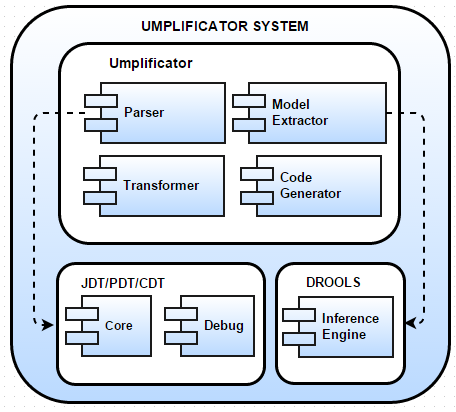
\includegraphics[width=0.75\textwidth]{Figures/UmplificatorComponents.png} 
\caption{The Umplificator components}
\label{fig:architecture}
\end{figure}

The mapping rules and rule engine are introduced in the following sub-section. 

\begin{figure}[h]
\centering
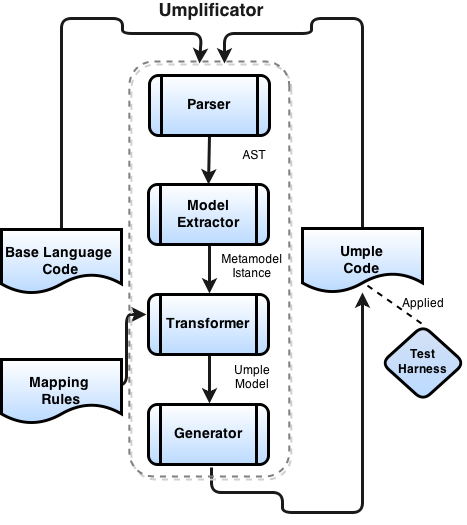
\includegraphics[width=0.75\textwidth]{Figures/Umplificator_ProcessFlow.png} 
\caption{The umplification process flow}
\label{fig:process_flow}
\end{figure}

\subsection{Rule Based Language}
The rule engine interprets and executes the mapping rules on the source model and target model to produce the umplified version of the target model.
The Drools engine used by the Umplificator is composed of an inference engine that is able to scale to a large number of rules and facts.  The inference component matches facts and data (base language models) against rules to infer conclusions, which result in actions (model transformations). A rule is a two-part structure (LHS and RHS) using first order logic for reasoning over knowledge representation. Pattern matching is performed to match facts against rules and is implemented using the Rete algorithm [15]. The rule engine is initialized with the rules. A Drools rule has the basic form: 

\begin{lstlisting}[language={drools},label={lst:drools}, caption=Basic rule in Drools] 
rule "name" 
  when LHS then RHS
end
\end{lstlisting}


where LHS is the conditional part of the rule and RHS is a block that allows dialect-specific semantic code to be executed. 
The rules are grouped in files for each of the cases (levels of refactoring) discussed earlier. In other words, there is a rule file containing rules, functions and queries to transform variables into attributes, another file containing those to transform variables into associations and so on. 
The rules as explained in this paper are instructions indicating how a piece of the Base language model (Java Model, C++ model, etc.) is mapped to a piece of an Umple model. Additionally, in Drools, one can specify:
\begin{itemize}
\item \textbf{Functions}: These are used for invoking actions on the consequence (then) part of the rule, especially if that particular action is used over and over again. In the Umplificator, functions are used instead of helper classes so the logic is kept in one place.
\item \textbf{Queries}: These provide a means to search working memory and store the results under a named value. In the Umplificator, they are used to gather metric information about the models analyzed. For instance, a query numberOfPublicMethods(..) returns the number of methods having 'public' as modifier. Queries do not have side effects, meaning that their evaluation cannot alter the state of the corresponding executing unit. 
\end{itemize}

In the Umplificator, the logic used for model transformations resides in the rules. Moreover, by using rules, we have a single point of truth, a centralized repository of knowledge. Rules can be also read and understood easily, so they can also serve as documentation.
Traditionally, rule engines have two methods of execution [16]: forward chaining and backward chaining. In forward chaining, the facts are asserted into working memory resulting in one or more rules being concurrently true and scheduled for execution. In backward chaining (goal driven), one starts with a conclusion, which the engine tries to satisfy. Drools is a Hybrid Chaining System because it implements both forward and back-ward mechanism. Our Umplificator uses the forward chaining method of operation in which the inference engine starts with facts, propagates through the rules, and produces a conclusion (e.g. a refactoring).  


As an example, consider the rules in Listing . The rule named transformImport(Lines 1-10) matches and converts any Import Declaration (Java Language) into an Umple depend construct. The dependency (Line 8) is then added to a matched Umple Class. The Umple Class is then put into the working memory (Line 9) so subsequent transformations can be made on the object (forward chaining). The rule named JavaFieldIsUmpleAttribute converts Java fields into basic Umple attributes. The attribute is then added to a matched Umple Class (Line 24). The attribute is put into the working memory (Line 25) so subsequent transformations can be made such as determining if the attribute is lazy or not. The rule named isLazyAttribute, not shown here, is used for this purpose. This rule matches and converts any basic attribute (in memory) that conforms to the required conditions into a lazy attribute (e.g. attribute.setIsLazy(true)). The complete set of mapping rules for the umplificator can be found at the umple code repository [17].

\begin{lstlisting}[language={drools},label={lst:rule_import}, caption=Initial Refactoring Mapping Rules]
 rule  "transform_Import"
 when
  import: ImportDeclaration();
  uClass: UmpleClass() ;
 then
  Depend depend = new Depend(getImportName(import));
  uClass.addDepend(depend);
  insert(uClass);
end
\end{lstlisting}



